\documentclass[border=0pt]{standalone}
\usepackage{fontspec}
\usepackage{tikz}
\usetikzlibrary{arrows.meta,positioning,backgrounds,fit,calc}

% --- professional, restrained palette ---
\definecolor{ink}{HTML}{1E293B}
\definecolor{sub}{HTML}{64748B}
\definecolor{page}{HTML}{FFFFFF}
\definecolor{card}{HTML}{F8FAFC}
\definecolor{line}{HTML}{CBD5E1}
\definecolor{app}{HTML}{2563EB}
\definecolor{vpn}{HTML}{0D9488}
\definecolor{hev}{HTML}{4F46E5}
\definecolor{tor}{HTML}{7C3AED}
\definecolor{net}{HTML}{059669}
\definecolor{fb}{HTML}{334155}
\definecolor{warn}{HTML}{B45309}

% text macros used inside nodes
\newcommand{\hd}[1]{{\bfseries #1}}
\newcommand{\subt}[1]{{\scriptsize\color{sub} #1}}

% back-to-front: page card (bg2) behind the app container (bg) behind nodes (main)
\pgfdeclarelayer{bg}\pgfdeclarelayer{bg2}\pgfsetlayers{bg2,bg,main}

\begin{document}
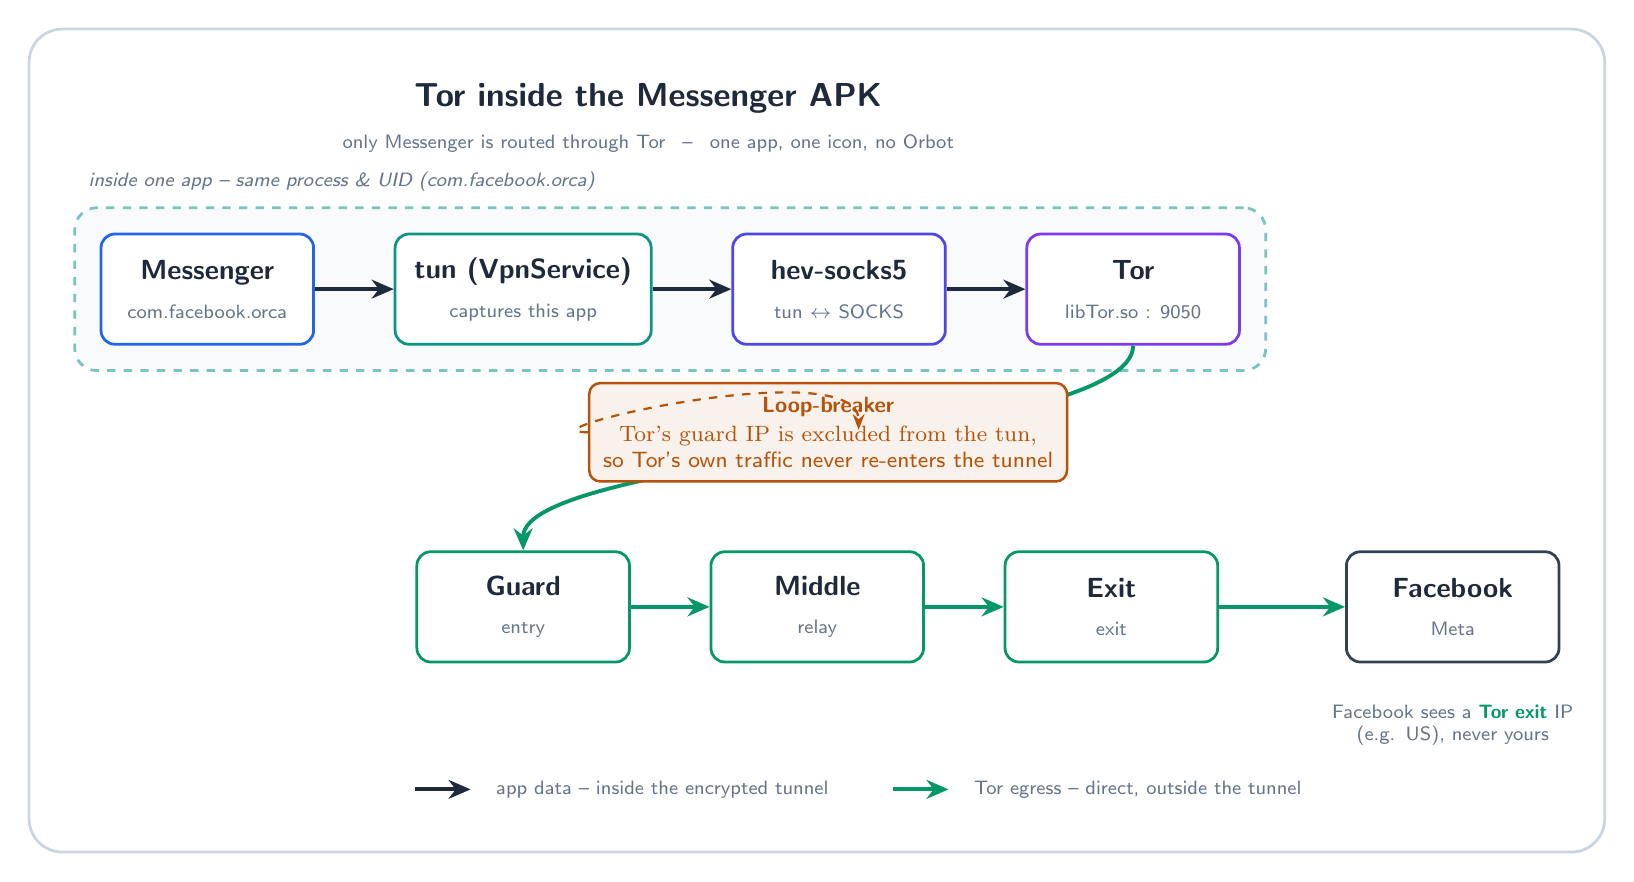
\begin{tikzpicture}[
  font=\sffamily,
  node distance=10mm,
  box/.style={rounded corners=5pt, draw=#1, line width=1pt, fill=white, text=ink,
              align=center, inner sep=7pt, minimum width=27mm, minimum height=14mm},
  sublbl/.style={font=\sffamily\scriptsize, text=sub},
  data/.style={-{Stealth[length=2.8mm,width=2.4mm]}, line width=1.4pt, draw=ink},
  egress/.style={-{Stealth[length=2.8mm,width=2.4mm]}, line width=1.4pt, draw=net},
]

% ============ TITLE ============
\node[font=\sffamily\large\bfseries, text=ink] (h1) {Tor inside the Messenger APK};
\node[sublbl, below=1pt of h1] (h2)
  {only Messenger is routed through Tor \, -- \, one app, one icon, no Orbot};

% ============ ROW 1: inside the app (same UID) ============
\node[box=app, below=14mm of h1.south, xshift=-56mm] (msg) {\hd{Messenger}\\[2pt]\subt{com.facebook.orca}};
\node[box=vpn, right=of msg] (tun) {\hd{tun (VpnService)}\\[2pt]\subt{captures this app}};
\node[box=hev, right=of tun] (hev) {\hd{hev-socks5}\\[2pt]\subt{tun $\leftrightarrow$ SOCKS}};
\node[box=tor, right=of hev] (tor) {\hd{Tor}\\[2pt]\subt{libTor.so : 9050}};

\draw[data] (msg) -- (tun);
\draw[data] (tun) -- (hev);
\draw[data] (hev) -- (tor);

% dashed container: same process / same UID
\begin{pgfonlayer}{bg}
  \node[draw=vpn!55, dashed, line width=1pt, rounded corners=8pt, fill=card,
        inner sep=9pt, fit=(msg)(tun)(hev)(tor)] (appbox) {};
\end{pgfonlayer}
\node[font=\sffamily\scriptsize\itshape, text=sub, anchor=south west]
  at ([xshift=2pt,yshift=2pt]appbox.north west)
  {inside one app -- same process \& UID (com.facebook.orca)};

% ============ ROW 2: Tor network -> Facebook ============
\node[box=net, below=26mm of tun] (guard) {\hd{Guard}\\[2pt]\subt{entry}};
\node[box=net, right=of guard]     (relay) {\hd{Middle}\\[2pt]\subt{relay}};
\node[box=net, right=of relay]     (exit)  {\hd{Exit}\\[2pt]\subt{exit}};
\node[box=fb,  right=16mm of exit] (face)  {\hd{Facebook}\\[2pt]\subt{Meta}};

% Tor egress: Tor -> guard (curves down on the left of the network row)
\draw[egress] (tor.south) .. controls +(0,-12mm) and +(0,12mm) .. (guard.north);
\draw[egress] (guard) -- (relay);
\draw[egress] (relay) -- (exit);
\draw[egress] (exit) -- (face);

% loop-breaker callout, placed clearly in the open middle area
\node[rounded corners=4pt, draw=warn, line width=0.9pt, fill=warn!8, text=warn,
      align=center, font=\sffamily\footnotesize, inner sep=5pt]
      (lb) at ($(hev)!0.5!(relay) + (0,2mm)$)
  {\bfseries Loop-breaker\\[1pt]\normalfont Tor's guard IP is excluded from the tun,\\
   so Tor's own traffic never re-enters the tunnel};
\draw[-{Stealth[length=2mm]}, warn, line width=0.8pt, dashed]
  (lb.west) .. controls +(-10mm,0) and +(0,10mm) .. ($(tor.south)!0.45!(guard.north)+(0,1mm)$);

% caption under Facebook
\node[sublbl, below=4mm of face, align=center, text width=36mm]
  {Facebook sees a \textbf{\color{net}Tor exit} IP\\ (e.g. US), never yours};

% ============ legend ============
\node[sublbl, anchor=west] (lgAt) at ($(guard.south west)+(9mm,-16mm)$)
  {app data -- inside the encrypted tunnel};
\draw[data] ([xshift=-9mm]lgAt.west) -- ([xshift=-2mm]lgAt.west);
\node[sublbl, anchor=west] (lgBt) at ($(lgAt.east)+(16mm,0)$)
  {Tor egress -- direct, outside the tunnel};
\draw[egress] ([xshift=-9mm]lgBt.west) -- ([xshift=-2mm]lgBt.west);

% ============ background card ============
\begin{pgfonlayer}{bg2}
  \node[fill=page, draw=line, line width=1pt, rounded corners=12pt,
        fit=(h1)(h2)(appbox)(guard)(relay)(exit)(face)(lb)(lgAt)(lgBt), inner sep=16pt] {};
\end{pgfonlayer}
\end{tikzpicture}
\end{document}
